%% For the copyright see the source file.
\documentclass[acmtog]{acmart}

%% NOTE that a single column version is required for 
%% submission and peer review. This can be done by changing
%% the \doucmentclass[...]{acmart} in this template to 
%% \documentclass[manuscript,screen]{acmart}
%\AtBeginDocument{%
%  \providecommand\BibTeX{{%
%    \normalfont B\kern-0.5em{\scshape i\kern-0.25em b}\kern-0.8em\TeX}}}
%\setcopyright{acmcopyright}
%\copyrightyear{2023}
%\acmYear{2023}
%\acmDOI{XXXXXXX.XXXXXXX}
%\citestyle{acmauthoryear}

\begin{document}
\title{Optimizing Sales of Ducks and Fish}
\author{Patrick Lowe}
\email{lowe03@ads.uni-passau.de}
\affiliation{%
  \institution{University of Passau}
  \streetaddress{Innstr. 41}
  \city{Passau}
  \country{Germany}
  \postcode{94032}
}
%\renewcommand{\shortauthors}{ TEST LINE 35 TEST}

\begin{abstract}
This project looks at the reproducibility of Head First Data Analysis book (HFDA) sales optimization in chapter 3, and how to future proof the tools used. The Excel Solver used may not always be accessible, the challenge is to create an open-source alternative. While Google Sheets offers a similar solution, this project investigates the more widely accessible Python programming language and external package PuLP. This tool was able to replicate Excels Solver results, but with the added benefit of being more versatile (open-source, easily redistributed, more configurable). We also remark on the standard of artefacts available for reproducibility.
\end{abstract}

\keywords{optimization, python, excel solver, xls, reproducibility, docker}
\maketitle

\section{Introduction}
Is it possible to reproduce the results from chapter 3 of Head First Data Analysis on optimization? We use artefacts available from O'Reillys resource website to reproduce these results, first using Excels Solver add-on, then replicating the results using Python. We utilize the Python package PuLP for linear problem solving. It then looks at a pitfall, not recognising seasonal changes in sales. We predict these sales using historical data. Since they ask the reader to predict sales but also give suggested sales we perform both tasks. First replicating their suggested sales, then making our own analysis; which is also replicable for others. This project is held within a Docker container, allowing it to be used across different environments. The results may change only if new sales are added to the historical sales, the first and second analysis will always replicate to the HFDA values. There may be future limitations on reproducibility of this project if support for Python or its package versions are no longer supported. While the goal is to reproduce the results using the same tools, we used an alternative tool (Python) as Excel requires a license and is not provided as an artefact.

\section{Methodology}
Docker creates a reproducible environment so we can replicate the results of HFDA chapter 3 on optimization. Other alternatives like Podman and VirtualBox have more set-up than Docker. Docker is a widely used, open-source, virtual container which increases its chance of being available long term for future replications. The main challenge replicating the results and creating an environment which can continuously reproduce our own estimates on future sales. Since Excel requires a license to be run, we have opted to use Python as it is open source, requires minimal set-up, and has human-readable code. The docker file includes Ubuntu packages to create a \LaTeX\ compiler, the version of Python to use, and a requirements file to specify the version to use for each python package.

Initially, we created the Python script using Jupyter Notebooks for easy readability and corrections, however this is not used as part of the package. Instead, an export of the python script is used. This contains identical code but allows the script to be easily ran in docker. The Python package pandas is used to read the XLS data file and create a dataframe, the ceiling function of the math package rounds the predict sale of toys, matplotlib is used for the sales graph, OS is used to create the PDF report through pdflatex command, and the main package we use is PuLP. PuLP is a linear problem solver, which has a BSD license allowing for redistribution. Creating a function to run this means that any updates to the resources or profits could easily be adjusted in the excel file.

The challenges in replication were firstly understanding what the book had performed. We choose to reproduce their results by following the Excel Solver steps, but Solver no longer comes pre-installed and has to be manually added through the Addon manager. In selecting the constraints, the first 2 analysis are replicable but the 3rd is open to the reader, therefore we opted to get an average change in sales of both products between the months of December and January, each year. When using Solver, it produced 2 empty sheets which is seen in the XLS artefacts. This meant providing a named sheet when opening with Python. 

The only potential changes to the solver were the limits on productions, so a function was created to be called when needed, passing in 2 arguments; the upper limits on Fish and Ducks. The limitation in reproducibility is the final analysis which uses the readers prediction of values. For consistency, we opted to analyse the historical data sales. This section of code, input block 7 in the Python script, modifies 2 columns into a single, more readable column. The month column uses the first letter of the month, 'J' could be January or June or July. Since the file begins on January, and uses all months of the 3 years, we have changed the month to be the rows index + 1. So, January at index 0 now changes from 'J' to 1. This is normally not ideal when coding as the XLS file could easily change and skew the month numbers but this felt appropriate for a small dataset which is not going to change in a reproducibility test. 

Next, a dictionary containing the months of December and January for the years 2006 to 2008 was iterated over. It collects the sale of both products for that respective month, calculating the average change in sales from December to January to 2 decimal places. This average is used to predict the sales for the next month, January 2009. Finally, the predicted sales are added to the dataframe to be visualised using the matplotlib package. This graph contains 1 image with 3 lines representing the sale of fish, ducks and total sales, as in the book. We have highlighted the 3 categories more clearly, providing dates instead of letter, a clear legend, markers for our final sales, and an extra month of our predicted sales. The last line in this script uses the operating system package OS to call pdflatex, installed in Docker, producing a PDF \LaTeX\ report.

The script is able to reproduce the results of HFDA optimization chapter. Initially, following the steps with Excel also reproduced the results but creating an Excel macro to continuously reproduce the results and the graph is both tedious, and limiting (requiring manual intervention between steps). Python and Docker are an alternative which allows 1 step deployment while also having the opportunity to expand upon the steps in the book, if needed.

The artefact data could be stored better. The file has inconsistent layout, decorations, and different structured subsections that create a problem in reading the file to Python. This was resolved with slicing the pandas dataframe and storing the values into variables. An alternative would be hard coding the profits for each item, and The website for artefacts did not contain the instructions i.e. Chapter 3 of the book.  

\section{Results}
Overall, the project was replicable, but not reproducible. The artefacts site did not contain the instructions, Chapter 3 of the book, and had to be sourced elsewhere. Excel was also not provided and when locally installed the Solver add-on had to be manually added, which is not covered in the chapter. The data itself was fully available, and while having no impact on achieving results the structure could be improved. The first analysis uses 400 ducks and 300 fish as a limit. Our replication produces a profit of \$ 2320 which matches the profit in the book while also calculating identical limits, 80 fish and 400 ducks to be sold. 

The 2nd analysis replicates 150 ducks and 50 fish with a profit of \$ 950, again identical to the book. Although there are 2 analyses, we felt the book left it open to interpretation, that 50 fish and 150 ducks were suggestions. We analysed the average change in sales and predicted 98 fish and 133 ducks could be sold, for a profit of \$ 1057; slightly higher than what is estimated by HFDS. From the graph, we can see the sales seem to be climbing in comparison to the year previous.

\section{Figures}
\begin{figure}[h!]
  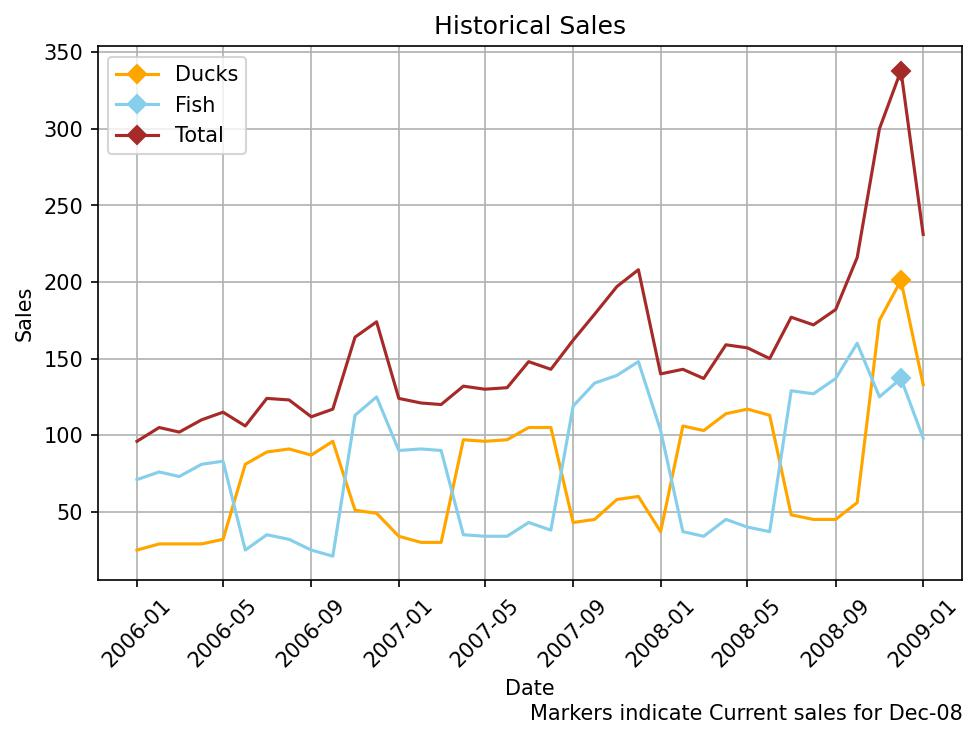
\includegraphics[width=\linewidth]{historic_sales.jpg}
  \caption{Sales of Ducks, Fish, and Total.}
  \label{fig:boat1}
\end{figure}

\begin{figure}[h!]
  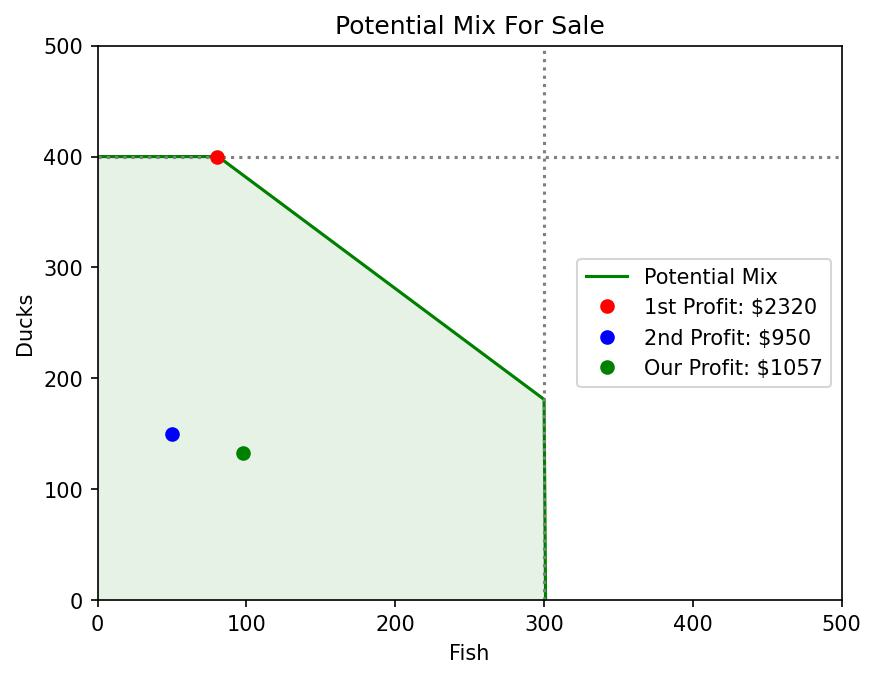
\includegraphics[width=\linewidth]{potential_mix.jpg}
  \caption{Potential Mix of Sales.}
  \label{fig:boat1}
\end{figure}

\section{Conclusions}
The project is not reproducible as access to Excel is limited, and support for Solver appears to be reducing as it is no longer a default add-on. Instead, it is replicable since we can use a new tool, Python, to produce identical results. On larger scale data, this new tool can be more efficient than Excel and easily updated or customised to better suit the users needs. The artefacts provided by HFDS were  reliable but could be improved. Namely, there were 2 blank sheets in the XLS files and also the website does not stick to a naming structure as it does with other chapters. A PDF of the chapter should also be provided as part of the artefacts.



\section{References}

* Github for continuing work
* Archive in Zenodo
* Conda for environment dependencies
* Docker for environment container

\end{document}
\endinput